%
% Documento: Disposições
%

\chapter{Framework Proposto}

    Neste capítulo irei abordar as tecnologias de utilizadas para a codificação do framework,
    detalhando os módulos e suas classes expostas para o usuário e as ferramentas utilizadas
    para controle de versão e publicação do framework.


    \section{Tecnologias Utilizadas}

        Para o desenvolvimento do framework foi utilizado apenas como linguagem para desenvolvimento o Python
        e para a manipulação e integração com o \emph{browser} a biblioteca em Python do Selenium \emph{Webdriver}. Por ser um
        projeto que visa ser o mais simples e leve possível apenas os módulos padrões do Python estão sendo utilizado
        para o desenvolvimento desta ferramenta.


        \subsection{Python}

            A escolha do Python \cite{Python} foi devida porque ele trata-se de uma linguagem de programação fácil de aprender e poderosa.
            Possuindo uma estruturas dados de alto nível e uma abordagem simples, mas eficaz, para a programação orientada
            a objetos. Contendo uma Sintaxe elegante e tipagem dinâmica, juntamente com uma interpretação natural, tornam
            a linguagem ideal para criação dos \emph{scripts} do Pybot.

        \subsection{Selenium WebDriver}
            \emph{Selenium Webdriver} \cite{webdriver} é um framework utilizado para se comunicar e enviar comandos para os \emph{browser}
            em conjunto com um controlador de cada \emph{browser} específico. Em comparação com seu antecessor, Selenium RC, o Selenium \emph{Webdriver}
            não precisa de um server para enviar os comandos para o \emph{browser}. Utilizando comando nativos do sistema operacional ao invés de
            comando javascript, usados pelo Selenium RC, deixam o Selenium \emph{Webdriver} uma excelente ferramenta para integração com diversos
            \emph{browser}.

        \subsection{Git e GitHub}
            Para o controle de versões e alterações do código fonte do framework e \emph{scripts} de exemplo foi utilizado a ferramenta
            Git \cite{git} em conjunto com os servidores do Github \cite{github} para hospedagem e gerenciamento. Com eles foi possível
            fazer alterações dos códigos fontes em qualquer computador e gerenciar os erros e melhorias do framework.


    \section{Módulos}

        O framework consiste em alguns módulos básicos, cada um com suas devidas utilidades e funções.
        A separação dos de cada módulos foi dada com base em suas caracteristicas e funcionalidades,

        \begin{figure}[H]
            \vspace*{0,3cm}
            \centering
            \caption{Diagrama de Componentes}
            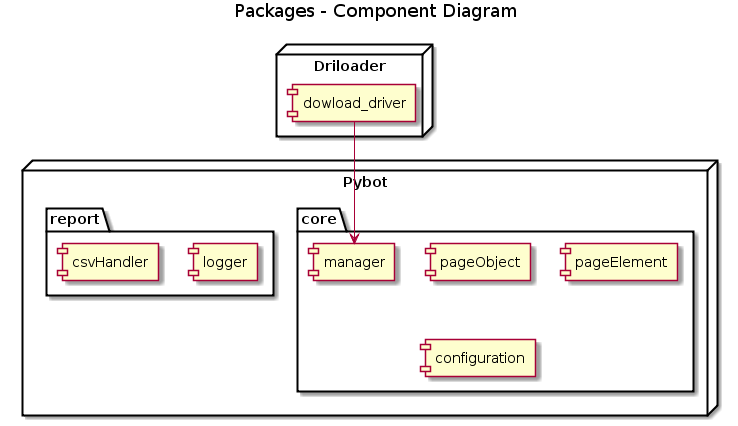
\includegraphics[width=1\textwidth]{./04-figuras/model}
            \label{fig:modules}
        \end{figure}

        \subsection{Core}
            Este módulo contém as funcionalidades básicas para a operação do framework com o Selenium \emph{Webdriver}
            e o gerenciamento dos parâmetros de execuções de cada script.

            \subsubsection{Manager}
            Manager server para abstrair o uso do Selenium \emph{Webdriver} criando uma camada de metodos própios fazendo com que caso alguma
            atualização da API do Selenium \emph{Webdriver} altere os \emph{scripts} criados não sejam impactados. Fazendo uso do Driloader mencionado na
            subseção \ref{driloader} ele verifica a necessidade do download do driver para poder executar o \emph{Selenium Webdriver}.

            \subsubsection{Configuration}
            Responsável por gerar as configurações básicas para o framework e disponibilizá-las no arquivo \emph{pybot.ini}.
            Este arquivo é criado para cada script do usuário e nele arquivo é possível adicionar qualquer tipo de configurações ou parâmetros
            necessárias para o usuário, apenas sendo preciso seguir os padrões descrito na imagem \ref{fig:pybot.ini} e utilizando com o comando
            \mbox{\emph{configuration.getConfig('Seção', 'variável')}}

            \begin{figure}[H]
                \vspace*{0,3cm}
                \centering
                \caption{Estrutura pybot.ini}
                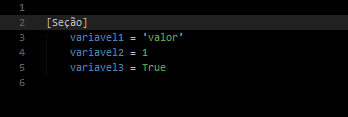
\includegraphics[width=0.7\textwidth]{./04-figuras/ini}
                \label{fig:pybot.ini}
            \end{figure}

        \subsection{Component}
        \label{Comp}
            Módulo criado para seguir os padrões de \emph{PageObject} e \emph{PageElement}, contendo abstração para os tipos de inputs do \emph{html}.

            \subsubsection{WebElement}
                Serve para abstrair o uso da classe WebElement do próprio Selenium Webdriver. Contendo uma classe para cada tipo de campo dos \emph{html},
                ele dispõe de algumas funcionalidades básica, como a atribuição de uma valor para um elemento do tipo \emph{input text} irá escrever
                valor dentro do campo, \emph{select} irá selecionar a opção cujo texto seja igual ao valor informado, \emph{radio} irá selecionar o
                a opção que tenha o \emph{value} do valor informado e para o tipo \emph{checkbox} irá marcar ou desmarcar as opções se o valor for
                verdadeiro(True) ou falso(False)

            \subsubsection{PageElement e PageElements}
            \label{PageElement}
                Essas classes servem para controlar os elementos mapeados das telas. Sempre quando serão acessadas a classe faz novamente a pesquisa
                do elemento em tela, prevenindo assim uma das exceções mais comum do Selenium Webdriver que é a \emph{StaleElementReferenceException},
                que é quando o elemento em questão não existe mais no DOM ou a referência que tinha não é mais a mesma. Conta com uma lista de seletores
                que facilitam para o usuário buscar os elementos e deixam o código mais legível. Usa-se a classe PageElements quando quiser pegar mais
                de um elemento com o mesmo seletor.

                \begin{figure}[H]
                    \vspace*{0,3cm}
                    \centering
                    \caption{Lista de Seletores}
                    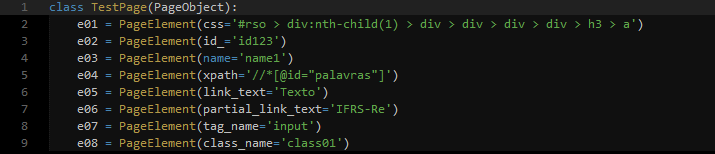
\includegraphics[width=1\textwidth]{./04-figuras/selectors}
                    \label{fig:selectors.png}
                \end{figure}

            \subsubsection{PageObject}
                Classe simbolica, serve apenas para poder juntar diversos PageElement descritos pelo usuário em uma classe para melhor
                legibilidade e componentização das páginas mapeadas.

        \subsection{Report}

            Estes módulo está destinado para geração de logs de execuções internas do framework, criação e controle
            de logs definidos pelos usuário e a criação de planilhas analíticas de dados extraídos das páginas.

            \subsubsection{Logger}
            Classe de geração dos Logs de execução do framework.

            \subsubsection{CsvHandler}
            Utilizado para geração de planilhas com dados extraídos das páginas para análise posterior do usuário.

        \subsection{Driloader}
        \label{driloader}
            Driloader é o responsavel pelo download dos driver de cada \emph{browser},suportando download dos driver do Internet Explorer,
            Firefox e Chrome, sendo possível para o usuário selecionar uma versão específica, a ultima versão ou detectar
            automaticamente qual a versão adequada para o \emph{browser} instalado do usuário. Como para utilização do Selenium
            Webdriver é necessário um driver específico de cada \emph{browser} foi tomada a decisão da criação desse projeto,
            inicialmente o Driloader era um módulo do framework mas pela autonomia e praticidade que ele proporciona aos
            usuários do Selenium Webdriver foi feita a separação dele do Pybot.



